% PFG Node Types visualization
% Shows the different node types and their relationships

\begin{figure}[t]
\centering
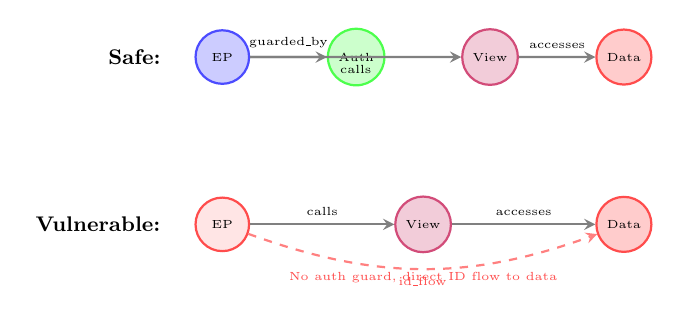
\begin{tikzpicture}[
    scale=0.85, transform shape,
    endpoint/.style={circle, draw=blue!70, fill=blue!20, thick, minimum size=0.8cm, font=\tiny},
    middleware/.style={circle, draw=green!70, fill=green!20, thick, minimum size=0.8cm, font=\tiny},
    data/.style={circle, draw=red!70, fill=red!20, thick, minimum size=0.8cm, font=\tiny},
    view/.style={circle, draw=purple!70, fill=purple!20, thick, minimum size=0.8cm, font=\tiny},
    arrow/.style={->, thick, >=stealth, draw=black!50},
    dasharrow/.style={->, thick, >=stealth, draw=red!50, dashed},
]

% Safe endpoint (top)
\node[endpoint] (ep1) at (0, 3) {EP};
\node[middleware] (mw1) at (2, 3) {Auth};
\node[view] (v1) at (4, 3) {View};
\node[data] (d1) at (6, 3) {Data};

\draw[arrow] (ep1) -- (mw1) node[midway, above, font=\tiny] {guarded\_by};
\draw[arrow] (ep1) -- (v1) node[midway, below, font=\tiny] {calls};
\draw[arrow] (v1) -- (d1) node[midway, above, font=\tiny] {accesses};

% Vulnerable endpoint (bottom)
\node[endpoint, draw=red!70, fill=red!10] (ep2) at (0, 0.5) {EP};
\node[view] (v2) at (3, 0.5) {View};
\node[data] (d2) at (6, 0.5) {Data};

\draw[arrow] (ep2) -- (v2) node[midway, above, font=\tiny] {calls};
\draw[arrow] (v2) -- (d2) node[midway, above, font=\tiny] {accesses};
\draw[dasharrow] (ep2) to[bend right=20] node[midway, below, font=\tiny, text=red!70] {id\_flow} (d2);

% Labels
\node[font=\small, anchor=east] at (-0.8, 3) {\textbf{Safe:}};
\node[font=\small, anchor=east] at (-0.8, 0.5) {\textbf{Vulnerable:}};
\node[font=\tiny, text=red!70] at (3, -0.3) {No auth guard, direct ID flow to data};

\end{tikzpicture}
\caption{Comparison of safe vs. vulnerable endpoint subgraphs in a PFG. The safe endpoint has an authentication guard between it and data access; the vulnerable endpoint exposes a direct identifier flow without authorization.}
\label{fig:pfg-example}
\end{figure}
